\documentclass[aspectratio=169,11pt]{beamer}

\usepackage{graphicx}
\usepackage{tikz}
\usetikzlibrary{positioning,arrows.meta}
\usepackage{xcolor}
\usepackage{booktabs}
\usepackage{tabularx}
\usepackage{array}
\usepackage{ragged2e}

\definecolor{GEUBlue}{RGB}{20,55,105}
\definecolor{GEULightBlue}{RGB}{238,244,251}
\definecolor{GEUGrey}{RGB}{90,90,90}
\definecolor{GEULightGrey}{RGB}{245,246,248}

\usetheme{default}
\setbeamertemplate{navigation symbols}{}
\setbeamertemplate{blocks}[rounded][shadow=false]
\setbeamercolor{normal text}{fg=black,bg=white}
\setbeamercolor{frametitle}{fg=GEUBlue}
\setbeamercolor{structure}{fg=GEUBlue}
\setbeamercolor{block title}{fg=GEUBlue,bg=GEULightBlue}
\setbeamercolor{block body}{fg=black,bg=GEULightBlue}
\setbeamerfont{frametitle}{size=\Large,series=\bfseries}

% Replace with the actual logo filename
\newcommand{\GEULogo}{graphicera_logo.png}

% Header and footer
\setbeamertemplate{headline}{%
  \begin{tikzpicture}[remember picture,overlay]
    \node[anchor=north east,xshift=-0.30cm,yshift=-0.12cm]
      at (current page.north east)
      {\includegraphics[height=0.62cm]{\GEULogo}};
  \end{tikzpicture}
  \vspace{0.72cm}
}
\setbeamertemplate{frametitle}{%
  \vspace{0.03cm}
  \insertframetitle\par
  \vspace{0.04cm}
  \textcolor{GEUBlue}{\rule{\textwidth}{0.9pt}}
  \vspace{0.03cm}
}
\setbeamertemplate{footline}{%
  \leavevmode
  \hbox{%
  \begin{beamercolorbox}[wd=.82\paperwidth,ht=0.32cm,dp=0.10cm,leftskip=.3cm]{author in head/foot}
    \tiny Department of Computer Science \& Engineering | Graphic Era (Deemed to be University)
  \end{beamercolorbox}%
  \begin{beamercolorbox}[wd=.18\paperwidth,ht=0.32cm,dp=0.10cm,rightskip=.3cm]{date in head/foot}
  \end{beamercolorbox}}
}

\newcommand{\smallnote}[1]{\vspace{0.08cm}{\scriptsize\color{GEUGrey}#1}}
\newcommand{\placeholder}[1]{\textit{\color{GEUGrey}#1}}

\title{\textbf{Project-Based Learning}\\[2mm]\large Phase-I Evaluation}
\author{\textbf{Project Title}\\Team ID: DSCPP-III-2026-T198}
\institute{Department of Computer Science \& Engineering\\Graphic Era (Deemed to be University), Dehradun}
\date{Academic Session 2026--27}

\begin{document}

% 1
\begin{frame}[plain]
\begin{tikzpicture}[remember picture,overlay]
\draw[GEUBlue,line width=3pt] (current page.north west) -- (current page.north east);
\node[anchor=north east,xshift=-0.45cm,yshift=-0.35cm] at (current page.north east)
{\includegraphics[height=1.0cm]{\GEULogo}};
\node[align=center,text width=.84\paperwidth] at ([yshift=.25cm]current page.center)
{{\color{GEUBlue}\fontsize{26}{30}\selectfont\bfseries PROJECT-BASED LEARNING}\\[3mm]
 {\fontsize{18}{22}\selectfont PHASE-I EVALUATION}\\[7mm]
 {\color{GEUGrey}\Large\bfseries \placeholder{VidOptix – Video Compression System}}\\[3mm]
 {\color{GEUBlue}\normalsize Team ID: DSCPP-III-2026-T198}};
\node[align=center,anchor=south,yshift=.42cm] at (current page.south)
{\bfseries Department of Computer Science \& Engineering\\
Graphic Era (Deemed to be University), Dehradun\\[-1mm]
\scriptsize Academic Session 2026--27};
\end{tikzpicture}
\end{frame}

% 2
\begin{frame}{Team \& Mentor Details}
\begin{columns}[T,totalwidth=\textwidth]
\column{.48\textwidth}
\begin{block}{Team Information}
\begin{tabular}{@{}ll@{}}
\textbf{Team ID:} & DSCPP-III-2026-T198\\
\textbf{Semester:} & 3rd \\
\textbf{Section:} & B,DS1,ML1,ML2\\
\textbf{Domain:} & \placeholder{Data Structure and C++}
\end{tabular}
\end{block}
\column{.48\textwidth}
\begin{block}{Team Members}
1.\quad \placeholder{Anshika Goswami -- 2510380062}\\
2.\quad \placeholder{Yaduveer Yadav -- 2510370438}\\
3.\quad \placeholder{Deepanshi Choudhary -- 2510370456}\\
4.\quad \placeholder{ Mohd Ubaid -- -2510370084}
\end{block}
\end{columns}
\vspace{2mm}
\begin{block}{Mentor}
\placeholder{Mr. Kartikey Arora}
\hfill
\textbf{Interactions completed: 4} 
\end{block}
\end{frame}

% 3
\begin{frame}{Problem Statement \& Motivation}

\begin{block}{Problem Statement}

\footnotesize

\placeholder{
Nowadays, videos are used everywhere, from social media to online classes.
The main issue is that video files take up a lot of storage space and require
more internet bandwidth to share or stream. In addition, some videos have
problems like low brightness, poor contrast, or unwanted noise. Our project
focuses on improving video quality while also reducing the file size.
}

\end{block}

\vspace{-2mm}

\begin{columns}[T,totalwidth=\textwidth]

\column{.50\textwidth}

{\footnotesize
\textbf{\color{GEUBlue}Motivation}
}

\vspace{0.2mm}

\begin{itemize}

\setlength{\itemsep}{0pt}
\setlength{\parskip}{0pt}

\footnotesize

\item
\placeholder{
Large videos are difficult to store and share.
}

\item
\placeholder{
Poor-quality videos affect the viewing experience.
}

\item
\placeholder{
Existing compression systems are complex and not easy for students to understand.
}

\item
\placeholder{
We wanted to build a project that helps us learn how video enhancement
and compression work in practice.
}

\end{itemize}


\column{.45\textwidth}

{\footnotesize
\textbf{\color{GEUBlue}Target Users / Stakeholders}
}

\vspace{0.2mm}

\begin{itemize}

\setlength{\itemsep}{0pt}

\footnotesize

\item
\placeholder{Content creators}

\item
\placeholder{Students learning multimedia processing}

\item
\placeholder{Social media users}

\item
\placeholder{Organizations managing video archives}

\end{itemize}

\end{columns}

\end{frame}

% 4
\begin{frame}{Objectives}
\textbf{\color{GEUBlue}Project Objectives}
\vspace{1mm}
\begin{enumerate}\itemsep0pt
\item \placeholder{Create a video enhancement and compression system using C++..}
\item \placeholder{Process videos one frame at a time.}
\item \placeholder{Improve video quality using basic enhancement techniques.}
\item \placeholder{Reduce file size using compression methods.}
\item \placeholder{Efficient video compression and enhancement for easier storage,sharing and streaming.}
\end{enumerate}
\vspace{0.5mm}

\begin{center}

\colorbox{GEULightBlue}
{
\parbox{.88\textwidth}
{
\scriptsize

\textbf{Key Objective:}

\begin{itemize}

\setlength{\itemsep}{0.2pt}
\setlength{\leftmargini}{1.2em}

\scriptsize

\item
Achieve meaningful video size reduction while maintaining acceptable visual quality.

\item
Providing performance statistics such as compression ratio and processing time.

\item
To reduce video size while keeping the quality good enough for normal viewing.

\item
To display useful results such as compression ratio and processing time.

\end{itemize}

}
}

\end{center}

\end{frame}



% 5
\begin{frame}{Proposed Solution}
\begin{columns}[T,totalwidth=\textwidth]
\column{.49\textwidth}
{\small\textbf{\color{GEUBlue}Proposed Approach}}
\vspace{0.2mm}
\begin{enumerate}
\setlength{\itemsep}{0pt}
\small
\item \placeholder{Take a video as input.}
\item \placeholder{Extract frames from the video.}
\item \placeholder{Improve brightness, contrast, and reduce noise.}
\item \placeholder{Apply DCT and Quantization.}
\item \placeholder{Use Zig-Zag Scanning and RLE.}
\item \placeholder{Perform Huffman Coding for further compression.}
\item \placeholder{Generate the final compressed output along with statistics.}
\end{enumerate}
\column{.47\textwidth}
{\small\textbf{\color{GEUBlue}Key Features}}
\vspace{0.2mm}
\begin{itemize}
\setlength{\itemsep}{0pt}
\small
\item \placeholder{Video Frame Extraction}
\item \placeholder{Video Enhancement}
\item \placeholder{DCT-Based Compression}
\item \placeholder{Huffman Coding}
\item \placeholder{Compression Statistics Dashboard}
\end{itemize}
\end{columns}
\vspace{0.5mm}
\begin{center}
{\scriptsize\textit{\color{GEUGrey}
The system improves video quality and simultaneously reduces storage requirements using multiple compression stages while preserving acceptable visual quality.}}
\end{center}
\end{frame}
% 6
\begin{frame}{Integration of PBL Course Concepts}
\begin{center}
\scriptsize
\renewcommand{\arraystretch}{1.20}
\begin{tabularx}{.94\textwidth}{@{}>{\bfseries}p{2.45cm}>{\RaggedRight\arraybackslash}X>{\RaggedRight\arraybackslash}p{3.05cm}@{}}
\toprule
Course & Concepts Applied & Project Module\\
\midrule
Data Structures in C &
\placeholder{Queue, Priority Queue (Min Heap), Binary Tree, Vectors} &
\placeholder{Frame Processing, Huffman Coding, Data Storage}\\[1mm]
OOPs with C++ &
\placeholder{Classes, Objects, Encapsulation, Constructors, File Handling} &
\placeholder{Video, Frame, Enhancer, Compressor, HuffmanCoder Classes}\\
\bottomrule
\end{tabularx}
\end{center}
\vspace{2mm}
\begin{center}
\colorbox{GEULightBlue}{\parbox{.88\textwidth}{\small
\textbf{Requirement:}
Our project meaningfully integrates both subjects because the entire system is built using OOP classes, while the internal processing relies on Data Structures such as Queue, Vector, Priority Queue, and Binary Tree. OOP organizes the system, and Data Structures enable efficient frame processing and Huffman compression.}}
\end{center}
\end{frame}

% 7
\begin{frame}
{System Architecture / Workflow}
\begin{center}
\resizebox{.96\textwidth}{!}{
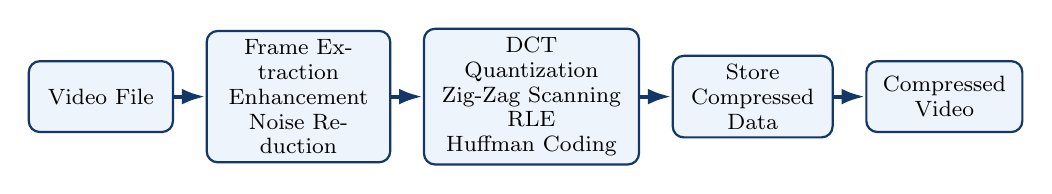
\begin{tikzpicture}[
box/.style={rectangle,rounded corners=4pt,draw=GEUBlue,fill=GEULightBlue,
line width=.8pt,align=center,font=\fontsize{8}{9}\selectfont,
inner xsep=4pt,inner ysep=3pt,minimum height=9mm},
arrow/.style={-{Latex[length=3mm,width=2mm]},draw=GEUBlue,line width=1.5pt}
]
\node[box,text width=1.55cm] (a) {Video File};
\node[box,text width=2.05cm,right=4mm of a] (b) {Frame Extraction\\Enhancement\\Noise Reduction};
\node[box,text width=2.45cm,right=4mm of b] (c) {DCT\\Quantization\\Zig-Zag Scanning\\RLE\\Huffman Coding};
\node[box,text width=1.75cm,right=4mm of c] (d) {Store Compressed\\Data};
\node[box,text width=1.70cm,right=4mm of d] (e) {Compressed Video};
\draw[arrow] (a.east) -- (b.west);
\draw[arrow] (b.east) -- (c.west);
\draw[arrow] (c.east) -- (d.west);
\draw[arrow] (d.east) -- (e.west);
\end{tikzpicture}}
\end{center}
\vspace{-1mm}

\begin{columns}[T,totalwidth=\textwidth]

\column{.49\textwidth}

{\small
\textbf{\color{GEUBlue}Major Components}
}

\begin{itemize}

\setlength{\itemsep}{0pt}

\tiny

\item
\textbf{Video \& Frame Module}
-- Loads video and extracts frames sequentially.

\item
\textbf{Enhancement Module}
-- Adjusts brightness/contrast and reduces noise.

\item
\textbf{Transform \& Quantization}
-- Applies DCT and quantization to reduce redundancy.

\item
\textbf{Zig-Zag \& RLE}
-- Reorders coefficients and encodes repeated values efficiently.

\end{itemize}
\column{.47\textwidth}

{\small
\textbf{\color{GEUBlue}}Data/Control Flow
}

\begin{itemize}

\setlength{\itemsep}{0pt}

\tiny

\item
\textbf{Huffman Coding}
-- Builds a Huffman tree and generates variable-length codes.

\item
\textbf{Storage / Output}
-- Stores compressed data and creates the final output.

\item
\textbf{Statistics / Evaluation}
-- Reports sizes, compression ratio, and processing time.

\item
\textbf{OOP Controller / File Handling}
-- Coordinates Video, Frame, Enhancer, Compressor, and HuffmanCoder classes.
\end{itemize}
\end{columns}
\end{frame}

% 8
\begin{frame}{Technology Stack \& Methodology}

\begin{columns}[T,totalwidth=\textwidth]

\column{.48\textwidth}

\begin{block}{Technology Stack}

\tiny

\begin{itemize}

\setlength{\itemsep}{0.5pt}

\item
\textbf{C++:}
High performance, OOP support, and STL data structures.

\item
\textbf{OpenCV:}
Frame extraction, video I/O, and image enhancement.

\item
\textbf{Data Structures:}
Queue, Vector, Priority Queue (Min Heap), Binary Tree.

\item
\textbf{File Handling:}
C++ streams for reading/writing project data and output.

\item
\textbf{VS Code:}
Development and debugging environment.

\item
\textbf{GitHub:}
Version control and team collaboration.

\end{itemize}

\end{block}


\column{.48\textwidth}

\begin{block}{Development Methodology}

\tiny

\begin{enumerate}

\setlength{\itemsep}{0.5pt}

\item
\textbf{Requirement Analysis}
-- define enhancement, compression, and evaluation needs.

\item
\textbf{Algorithm Study}
-- study DCT, Quantization, RLE, Huffman Coding, and enhancement methods.

\item
\textbf{System Design}
-- define modules, classes, data structures, and workflow.

\item
\textbf{Implementation}
-- develop frame, enhancement, compression, storage, and statistics modules.

\item
\textbf{Testing \& Evaluation}
-- compare size, time, and output quality.

\item
\textbf{Refinement}
-- improve performance and the quality/compression balance.
\end{enumerate}

\end{block}

\end{columns}


\vspace{0.5mm}
\smallnote{C++ provides high performance and supports both OOP and Data Structures. OpenCV simplifies video frame processing and enhancement operations.}
\end{center}
\end{frame}

% 9
\begin{frame}{Initial Progress \& Team Contribution}

\begin{columns}[T,totalwidth=\textwidth]

\column{.43\textwidth}

{\small
\textbf{\color{GEUBlue}Progress Achieved}
}

\begin{itemize}

\setlength{\itemsep}{2pt}

\small

\item
\placeholder{Literature review completed.}

\item
\placeholder{Compression algorithms studied.}

\item
\placeholder{System architecture prepared.}

\item
\placeholder{Workflow finalized.}

\item
\placeholder{Technology stack selected.}

\end{itemize}


\column{.54\textwidth}

{\small
\textbf{\color{GEUBlue}Individual Contribution}
}

\vspace{1mm}

\scriptsize

\renewcommand{\arraystretch}{1.10}

\begin{tabularx}{\textwidth}
{
@{}
p{1.55cm}
p{1.55cm}
X
@{}
}

\toprule

Member
&
Role
&
Contribution
\\

\midrule

\placeholder{Anshika Goswami}
&
\placeholder{Team and Project Lead}
&
\placeholder{
Planning, Structuring the project
}
\\

\placeholder{Yaduveer Yadav}
&
\placeholder{Module Planner}
&
\placeholder{
Research,Module Identification
}
\\

\placeholder{Deepanshi Choudhary}
&
\placeholder{Report and Presentation}
&
\placeholder{
Documentation,Research
}
\\

\placeholder{Mohd Ubaid}
&
\placeholder{Project Planner}
&
\placeholder{
Idea Initiation,Work Flow 
}
\\

\bottomrule

\end{tabularx}

\end{columns}

\end{frame}


% 10
\begin{frame}{Roadmap, Expected Outcomes \& References}

\begin{columns}[T,totalwidth=\textwidth]

\column{.47\textwidth}

{\small
\textbf{\color{GEUBlue}Roadmap}
}

\begin{itemize}

\setlength{\itemsep}{0.8pt}

\scriptsize

\item
\textbf{Phase-I:}
Proposal, requirements, literature review,
architecture, and design.

\item
\textbf{Phase-II:}
Module implementation, integration,
testing, and evaluation.

\item
\textbf{Phase-III:}
Optimization, final prototype,
documentation, and demonstration.

\end{itemize}

\vspace{0.4mm}

{\small
\textbf{\color{GEUBlue}Expected Outcomes}
}

\begin{itemize}

\setlength{\itemsep}{0.5pt}

\tiny

\item
Working video enhancement and compression prototype

\item
Measurable reduction in video storage size

\item
Acceptable visual quality after processing

\item
Compression ratio and processing-time report

\item
Scalable for real time processing and cloud deployment

\end{itemize}


\column{.47\textwidth}

{\small
\textbf{\color{GEUBlue}References}
}

\begin{itemize}

\setlength{\itemsep}{1pt}

\tiny

\item
\href{
https://docs.opencv.org/4.x/
}{
OpenCV Documentation
}

\item
\href{
https://opencv.org/
}{
OpenCV Official Website
}

\item
\href{
https://www.nist.gov/dads/
}{
NIST Dictionary of Algorithms and Data Structures
}

\item
\href{
https://nvlpubs.nist.gov/nistpubs/Legacy/SP/nbsspecialpublication500-12.pdf
}{
NIST Data Compression Reference
}

\item
\href{
https://mathworld.wolfram.com/HuffmanCoding.html
}{
Wolfram MathWorld -- Huffman Coding
}

\end{itemize}

\vspace{0.3mm}

{\scriptsize
\color{GEUGrey}
\textit{
Click any reference title to open the corresponding website/document.
}
}

\vfill

\begin{center}

\colorbox{GEUBlue}
{
\parbox{.78\textwidth}
{
\centering
\color{white}
\textbf{Thank You}
\\
Questions \& Suggestions
}
}

\end{center}

\end{columns}

\end{frame}


\end{document}















